\section{Parámetros de la ecuación de estado cúbica}

El cálculo de los parámetros depende de la cantidad de compuestos presentes en el sistema.

\begin{itemize}
 \item Para los compuestos puros la clase `Substance' define el cálculo de los parámetros usando una expresión de $\alpha$ , los parámetros $\Omega_a$ y $\Omega_b$ de la ecuación de estado y las propiedades del compuesto puro.
 \item Para las mezclas, la clase `Mixture' define el cálculo de los parámetros usando una regla de mezclado y el cojunto de los parámetros  $a$ y $b$ calculados a partir de los compuestos puros.
\end{itemize}




Esta estructura se muestra en laf figura \ref{fig:homogeneousCalculations}

\begin{figure}[!h]
  
  \centering
    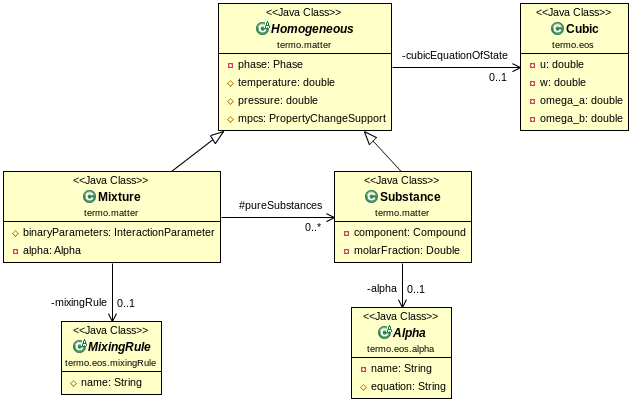
\includegraphics[scale=0.7]{homogeneousCalculations.png}
    \caption{Estructura de la librería para el cálculo de propiedades.}
    \label{fig:homogeneousCalculations}
\end{figure}

Nótese de la figura \ref{fig:homogeneousCalculations} los siguiente:
\begin{itemize}
	\item Que la clase `Homogeneous' contiene una ecuación del tipo `Cubic'.
 	\item Que las clases `Substance' y `Mixture' heredan las propiedades de la clase `Homogenous', como la ecuación cúbica, y puede hacer uso de ella.

\end{itemize}

	Cualquiera de las dos implementaciones de la clase `Homogeneous' tiene los métodos necesarios para calcular los parámetros de la ecuación cúbica según el código \ref{lst:homogeneousParameters}.

\begin{lstlisting}[caption=Cualquier objeto tipo `Homogeneous' puede calcular los parámetros de la ecuación de estado cúbica a y b, label={lst:homogeneousParameters}]
	Homogeneous system = ...// Objeto tipo `Homogeneous'.
	double a = system.calculate_a_cubicParameter();
	double b = system.calculate_b_cubicParameter();
\end{lstlisting}


\subsection{Compuesto puro}

Como se muestra en la figura \ref{fig:homogeneousCalculations} la clase `Substance' continene una expresión de $\alpha$, y una ecuación de estado, necesarias para realizar el cáculo de los parámetros, segun las ecuaciones \ref{eq:a} y \ref{eq:b}. 

\begin{equation}\label{eq:a}
	b_i = \Omega_b \frac{R T_{ci}}{p_{ci}} 
\end{equation}

\begin{equation}\label{eq:b}
 a_i = \Omega_a \frac{\left(R T_{ci}\right)^2}{p_{ci}} \alpha_i
\end{equation}

La expresión de $\alpha$ puede ser una función de la temperatura, las expresiones implementadas en el presente trabajo se muestran en la tabla \ref{tab:alphas}.

\begin{table}
\centering
\begin{tabular}{|c |c|c| }
	\hline
	Expresión & Parámetros & Ecuación de estado\\
	\hline
	Soave    &  ---& PR\\
	Peng and Robinson & ---& PR \\
	Mathias & $A$ & SRK\\
	Stryjek and Vera & $k_1$ & PRSV\\
	Adachi and Lu & $A,B$&SRK,PR\\
	Soave & $A,B$&SRK,PR\\
	Melhem, et al. & $A,B$&SRK,PR\\
	Androulakis et al. & $A,B,C$& SRK,PR\\
	Mathias and Copeman & $A,B,C$& SRK,PR\\
	Yu and Lu & $A,B,C$&SRK,PR\\
	Stryjek and Vera & $A,B,C$&PR\\
	Twu & $L,M,N$&TST\\
	Twu & ---&TST,PR\\
	GCEOS & ---& (Cualquier u y w)\\
	\hline
\end{tabular}
\caption{Expresiónes de $\alpha$ disponibles en la librería}\label{tab:alphas}
\end{table}


Para un compuesto puro los parámetros $a$ y $b$ se calculan segun el código \ref{lst:substanceParams}.


\begin{lstlisting}[caption={Cálculo de los parámetros para el Ciclohexano, con la ecuación de estado Soave Redlich Kwong y la expresión de $\alpha$ de mathias },label={lst:substanceParams}]
import.termo.eos.Cubic;
import.termo.eos.Alpha;
import.termo.component;
...
Compound compound = new Compound("Cyclohexane");
compound.setCriticalPressure(4073000);
compound.setCriticalTemperature(553.5);
compound.setAcentricFactor(0.211);

Cubic srk = EquationsOfState.redlichKwongSoave();
Alpha mathias = Alphas.getMathiasExpression();

Substance substance = new Substance(srk,mathias, compound,Phase.LIQUID);

double a = substance.calculate_a_cubicParameter();
double b = substance.calculate_b_cubicParameter();
\end{lstlisting}


Para realizar el cálculo es necesario definir las propiedades del compuesto, temperatura crítica, presión crítica, y algunas expresiones de $\alpha$ necesitan el factor acéntrico, para lo cual existe la clase `Compound' que encapsula todas las propiedades del compuesto.


En la sección \ref{subsec:pressure} se mostró como crear una ecuación de estado cúbica previamente definida, a través de la clase `EquatiosOfState'. Los valore de $\Omega_a$ y $\Omega_b$ se muestran en la tabla \ref{tab:cubics}. De forma muy similar al de las ecuaciońes de estado,la selección de la expresión de $\alpha$ se realiza a través de la clase `Alphas'.




\subsubsection{Mezcla}

El cálculo de los parámetros para una mezcla depende de la regla de mezclado, y en el caso de las reglas de mezclado basadas en la energía libre de exceso, también del modelo de actividad.

Las reglas de mezclado incluidas en este trabajo se muestran en la tabla \ref{tab:mixingrules}, y los modelos de actividad se listan en la tabla \ref{tab:activitymodels}.


\begin{table}
\begin{tabularx}{\textwidth}{|X|X|X|}
	\hline
	Regla & Parámetros & \\
	\hline
	Van Der Waals & $k_{ij}$ & $k_{ij} = k_{ji}$ \\
	Mathias-Klotz-Prausnitz& $k_{ij}$ & $k_{ij} \neq k_{ji}$ \\
	Huron Vidal & Según el model de actividad & \\
	Wong Sandler & $k_{ij}$ + los parámetros del modelo de actividad & $k_{ij} = k_{ji}$ \\
	\hline
\end{tabularx}
\caption{Reglas de mezclado implementadas}\label{tab:mixingrules}
\end{table}

\begin{table}
\begin{tabularx}{\textwidth}{|X|X|X|}
	\hline
	Modelo de actividad & Parámetros & \\
	\hline
	Wilson & $a_{ij}$, $b_{ij}$  & \\
	NRTL & $a_{ij}$, $b_{ij}$, $\alpha_{ij}$ & $\alpha_{ij} = \alpha_{ji}$ \\
	\hline
\end{tabularx}
\caption{Modelos de actividad }\label{tab:activitymodels}
\end{table}

El código \ref{lst:mixtureParameters} muestra el cálculo de los parámetros para una mezcla, donde la expresión de $\alpha$ es la misma para cada compuesto puro. 

\begin{lstlisting}[caption={Código para el cálculo de los parámetros de la ecuación de estado en una mezcla.}, label={lst:mixtureParameters} ]

Compound cyclohexane = new Compound("Cyclohexane");
cyclohexane.setCriticalPressure(4073000);
cyclohexane.setCriticalTemperature(553.5);
cyclohexane.setAcentricFactor(0.211);

Compound pentane = new Compound("N-pentane");
pentane.setCriticalPressure(3370000);
pentane.setCriticalTemperature(469.7);
pentane.setAcentricFactor(0.251);

Cubic equationOfState = EquationsOfState.pengRobinson();
Alpha alpha = Alphas.getMathiasAndCopemanExpression();

Mixture mixture = new MixtureBuilder()
			.addCompounds(cyclohexane,pentane)
			.setAlpha(alpha)
			.setEquationOfState(equationOfState)
			.setPhase(Phase.VAPOR)
			.build();

double a = mixture.calculate_a_cubicParameter();
double b = mixture.calculate_b_cubicParameter();
\end{lstlisting}

Es posible realizar el cálculo de los parámetros con una expresión de $\alpha$ diferente para cada compuesto puro según el código \ref{lst:mixtureParametersDifAlphas}. 


\begin{lstlisting}[caption={Código para el cálculo de los parámetros de la ecuación de estado en una mezcla, con diferentes expresiones de $\alpha$},label={lst:mixtureParametersDifAlphas}]
Mixture mixture = new MixtureBuilder()
			.addCompound(cyclohexane,Alphas.getPengAndRobinsonExpression())
			.addCompound(pentane,Alphas.getStryjekAndVeraExpression())
			.setEquationOfState(eos)
			.setPhase(phase)
			.setMixingRule(mixingRule)
			.setInteractionParameter(k)
			.build();

double a = mixture.calculate_a_cubicParameter();
double b = mixture.calculate_b_cubicParameter();
\end{lstlisting}
